\documentclass{article}
\usepackage[utf8]{inputenc}
\usepackage{url}
\usepackage{amsmath}
\usepackage{amssymb}
\usepackage{amsfonts}
\usepackage{graphicx}
\usepackage{hyperref}
\usepackage{cleveref}
\usepackage{tcolorbox}
\usepackage{booktabs}
\usepackage{siunitx}
\usepackage{subcaption}
\usepackage{gensymb}

% volume symbol
\makeatletter
\DeclareRobustCommand{\volume}{\text{\volumedash}V}
\newcommand{\volumedash}{%
  \makebox[0pt][l]{%
    \ooalign{\hfil\hphantom{$\m@th V$}\hfil\cr\kern0.08em--\hfil\cr}%
  }%
}
\makeatother

% todo boxes
\newtcbox{\todo}[1][yellow]{on line,arc=7pt,colback=#1!10!white,colframe=#1!50!black,before upper={\rule[-3pt]{0pt}{10pt}},boxrule=1pt, boxsep=0pt,left=6pt,right=6pt,top=2pt,bottom=2pt}



\title{Preliminary design of the battery cooling system for a electric racer airplane}
\author{Bernardo Bahia Monteiro\thanks{\url{b.b.monteiro@gmail.com}} \and
        Eli Yarson Nabham\thanks{\url{eli.yarson@gmail.com}} \and
        Mauro Cesar Vaz de Melo Junior \thanks{\url{emailmaurocesar@gmail.com}}\and
        Vitório Luiz Agostinho Fava\thanks{\url{vitorio.luizsf@gmail.com}}
        }
\date{\today}

\begin{document}

\maketitle

\begin{abstract}
    In this article we analyze various engineering solutions for battery pack cooling of a racer all electric aircraft. Starting from its thermal management system, in which will be taken in consideration its construction and operation characteristics, such as the materials with which it will be made and the environment conditions it will be subjected to.    
\end{abstract}

\section{Introduction}
\label{sec:intro}
 The Center of Aeronautical Studies (CEA) of the Federal University of Minas Gerais (UFMG) in Brazil was founded in 1964 with the aspiration to be a place where the students of Aeronautical Engineering could put in practice what they learn in class. The center was responsible for the design, construction and testing of more than ten flight proven airplanes throughout its history. It started by designing a glider for training, named Gaivota, seagull in Portuguese, then designing a high performance glider, transitioned to propelled aircraft during the eighties and now has its attention drawn specially to racer aircraft. The two newest designs, CEA308 and CEA311 (dubbed Anequim, the Portuguese name for the Mako shark), have the world record for the faster airplane under 300kg and 500kg of take-off wight, respectively. Now, CEA's newest endeavour in developing an all electrical racer airplane (\cref{fig:blueprint}). 
 
 \begin{figure}
     \centering
     \includegraphics[width=\textwidth]{fig/AZX02_AP.png}
     \caption{Blueprint of CEA's new electric racer airplane. Courtesy of Danilo Azevedo (\url{dcrazevedo@gmail.com}).}
     \label{fig:blueprint}
 \end{figure}
 
 Electric propulsion presents a different challenge from conventional propulsion. 
 Although modern electrical engines can be lighter and smaller than conventional ones for the same power output,
  energy storage with batteries is much more complicated than simply storing fuel. This paper attempts to solve one particular problem of energy storage in batteries for aeronautical: removing heat generated by the batteries. Unlike aviation fuel, batteries do heat up when discharging and this heat must be dissipated to avoid damaging the batteries, which have a strict operating temperature window.

In this paper, three different solutions for battery cooling are analyzed. 
Firstly, the simplest, cheapest and lightest solution possible: no cooling at all.
The heat from the battery is simply conducted out of the airframe by the fuselage itself. 
The drawback of this solution is very low capacity of heat extraction.
The second proposed solution is to remove heat by forced convection with outside air channeled via a NACA inlet or a ram inlet. 
This allows for much higher cooling rates with not much weight added. 
The NACA inlet also has the advantage of increasing drag only slightly.


%Outline (escrever descricao de cada secao)
This paper is organized as follows. 
\Cref{sec:methods} deals with the physical modelling of the two competing solutions. 
\Cref{sec:results} presents the preliminary design of each solution, that is,
    batteries operating temperature, and
    the drag and weight penalties incurred if a particular solution is chosen.
\Cref{sec:discussion} presents a in depth analysis of the results obtained 
and attempts to choose the best compromise, and
\cref{sec:conclusion} concludes this work.

\section{Methods}
\label{sec:methods}
%Uma secao para cada tipo de sistema. Escrever descricao do problema e equacionamento. As baterias podem ser modeladas como uma fonte de calor.

%Justificar que apenas a condicao de voo sera considerada porque o aviao e de bater recorde, entao ele nao precisa ficar parado no sol

For the purposes of a preliminary design,
 the battery system of the aircraft is modelled as a simple stedy state heat exchange system.
The batteries are assumed to be an uniform heat source of constant power output.
The flight situation considered is leveled flight at full power on a warm day (ISA$+10$), normal day (ISA) and cold day (ISA$-10$).

In this section, the heat conduction models for the two proposed solutions for cooling the batteries are explained, as well as the model for determining the heat output of the batteries.

\subsection{The battery}
\label{sec:battery}
There are three types of batteries cells commonly used in the industry, such as cylindrical, prismatic and pouch cells. 

Cylindrical cell still is one of the most used packaging style due to its easiness of manufacture and good mechanical stability. It doesn't have an ideal stacking profile, but its higher energy density compensates for this flaw and the empty space can be used for cooling in order to improve thermal management.The cylindrical cell is commonly used in portable applications and is also used in Tesla electric vehicles.

Prismatic cells make optimal use of space by using the layered approach, allowing flexible design. In contrast, it can be more expensive to manufacture, less efficient in thermal management and have a shorter life cycle than its cylindrical counterpart. Usually encased in aluminum or steel for stability, small amount of swelling must be accounted for.

Pouch cells offer simple, flexible lightweight solutions to battery design. Makes most efficient use of space, achieving up to 95\% packaging efficiency, however, swelling allowances must be made. It is light and cost-effective.\cite{packaging}
%Elaborate on witch one will be used on the article (explain why --- was it a project choice? cost choice? or it is still not decided --- can we make comparisons?)

As a project decision, battery packs consisting of state-of-the-art Lithium Sulfur technology pouch cells, from Oxisenergy will be used. \Cref{fig:pouch} shows one of these pouches and \cref{fig:pack} shows an assembled pack.

\begin{figure}
    \centering
    \begin{subfigure}{0.45\textwidth}
    \includegraphics[width=0.9\textwidth]{fig/pouch.jpg}
    \caption{pouch}
    \label{fig:pouch}
    \end{subfigure}
    \begin{subfigure}{0.45\textwidth}
    \centering
    \includegraphics[width=0.9\textwidth]{fig/pack.jpg}
    \caption{pack}
    \label{fig:pack}
    \end{subfigure}
    \caption{Li-S battery by Oxys Energy}
\end{figure}

\subsection{Thermal model of the battery}
The heat generation per unit volume of the battery can be calculated from the internal resistance of each battery cell.This is a simplified model, which takes in consideration only Joule heat, disregarding polarization and reaction heat, which are known to occur in Li-S batteries.\cite{samba2015battery}

Considering a series arrangement%
\footnote{This is without loss of generality. Considering a parallel arrangement would lead to the same result}%
, the joule heating of the battery is given by 
\begin{equation}
\label{eqn:Q1}
\dot{Q} =  N R_i I^2
\end{equation}
where $N$ is the number of cells, $R_i$ is the internal resistance of each cell and $I$ is the current flowing through the cell. Denoted the voltage supplied by each cell as $V_\text{cell}$ and the power required by the engine as $P$, the electrical current is given by
\begin{equation}
\label{eqn:current}
    I = \frac{P}{N V_\text{cell}}
\end{equation}

Combining \cref{eqn:Q1} and \cref{eqn:current}, the heat dissipated by the battery $\dot{Q}$ is
\begin{equation}
\dot{Q} = \frac{R_i}{N} \frac{P^2}{V_\text{cell}^2}
\end{equation}

Finally, since the number of batteries is given by the ratio of battery mass to cell mass, i.e.
\begin{equation}
N = \frac{m_b}{m_\text{cell}}
\end{equation}
the total heat dissipated is
\begin{equation}
    \dot{Q}=R_i \frac{m_\text{cell}}{m_b} \frac{P^2}{V_\text{cell}^2}
\end{equation}


\subsection{Conduction cooling}
\label{sec:cc}
In order to minimize the airplane's weight and drag, it is ideal to cool the batteries passively by heat conduction through the airplane's skin. The batteries would be attached to the lower surface of the wing, in order to avoid radiation heating and maximize the area available for heat transfer.

The heat transfer problem that arises from this configuration is shown in \cref{fig:conduction}. Heat is generated uniformly in the batteries' pouches, which are insulated on one side and in contact with the wing's skin on the other. The heat is then conducted through the skin and transferred by convection to the air passing by the wing.

 \begin{figure}
     \centering
     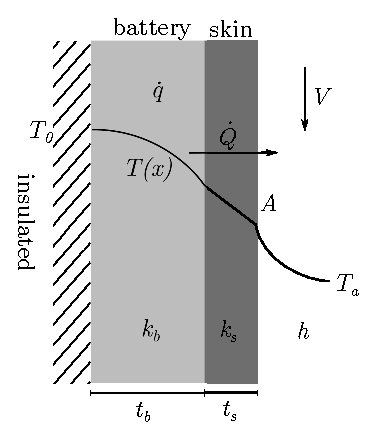
\includegraphics{fig/conduction.eps}
     \caption{Thermal system for conduction cooling}
     \label{fig:conduction}
 \end{figure}
 
 The equations that model this thermal system are
 \begin{align}
   T_0-T_{sb} &= \frac{\dot{q}}{2k_b}t_b^2 &\text{ for } 0 < x <t_b \\
   T_{sb}-T_{sa} &= \frac{\dot{Q}}{k_s A} t_s &\text{ for } t_b<x<t_b+t_s\\
   T_{sa} - T_a &= \frac{\dot{Q}}{hA} &\text{ for } x>t_b+t_s
 \end{align}
 where $T_0$ is the temperature at the insulated surface of the battery, $T_{sb}$ is the temperature at the battery-skin interface, $T_{sa}$ is the temperature at the skin-ambient interface and $T_a$ is the ambient temperature. $k_b$ and $k_s$ are the thermal conductivity of the battery and skin respectively, and $h$ is the convective coefficient of the air. $t_b$ and $t_s$ are the battery and skin thickness. $A$ is the surface area available for heat transfer, $\dot{Q}$ is the total heat flux generated by the battery, and $\dot{q}$ is the heat generated by unit of volume.
 
 Assuming uniform heat generation, i.e.\ $\dot{q} = \tfrac{Q}{At_b}$, these equations can be combined to relate the ambient temperature $T_a$ with the maximum temperature in the battery, $T_0$:
 \begin{equation}
    \label{eqn:conduction}
     T_0 = T_a + \frac{\dot{Q}}{A} \left(\frac{1}{h} + \frac{t_s}{k_s} + \frac{t_b}{2k_b} \right)
 \end{equation}
 
Alternatively, since the battery volume $\volume_b$ is known, the surface area can be expressed in terms of the battery thickness, i.e.\ $A = \frac{\volume_b}{t_b}$, or $Q/A = \dot{q} t_b$. Substituting this in \cref{eqn:conduction}, and doing some algebraic manipulation
\begin{equation}
    \frac{t_b^2}{2} + \left(\frac{k_b}{k_s} t_s + \frac{k_b}{h}\right) t_b - \frac{k_b}{\dot{q}}(T_0-T_a) = 0
\end{equation}

Solving for $t_b$ and choosing the positive root,
\begin{equation}
    t_b = t_s\left(\frac{k_b}{k_s} +\frac{k_b}{ht_s}\right)\left[\sqrt{1 + 2\left(\frac{k_b}{k_s} +\frac{k_b}{ht_s}\right)^{-2} \frac{T_0-T_a}{\dot{q}t_s}} - 1\right]
\end{equation}

The remaining step is to calculate the convection coefficient, $h$. For a high performance wing, a predominantly laminar boundary layer is expected. Kreith \cite{kreith} suggests the following relation for the local Nusselt number as a function of Reynolds and Prandtl numbers.
\begin{equation}
    Nu_x = 0.33\text{Re}_x^{1/2}\text{Pr}^{1/3}
\end{equation}
where the dimensionless coefficients are defined as follows
\begin{align}
\text{Nu} &= \frac{hx}{k} \\
\text{Re} &= \frac{\rho V x}{\mu} \\
\text{Pr} &= \frac{c_p \mu}{k}
\end{align}
$x$ is the chordwise dimension $k$ is the thermal conductivity, $\rho$ is air densisty, $V$ air speed, $c_p$ air specif heat at constant pressure, and $\mu$ is air's kinematic viscosity.

For getting a Nu valid for the entire wing, it is useful to consider $x=c/2$, where $c$ is the mean geometric chord. From Nu it is easy to calculate $h$.

\subsection{Air cooling}
\label{sec:air}
The most used system for cooling small aircraft generators and batteries is the air type. In this system, the battery pack is cooled by the stream of air forced through it by a pressure differential caused either by ram effect or a specially designed inlet, such as a NACA duct. In this subsection, the goal is to calculate the mass flow required for air cooling and the drag associated with it.

\begin{figure}
    \centering
    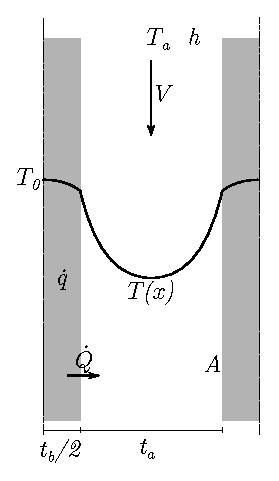
\includegraphics{fig/convection.eps}
    \caption{Thermal system for forced air convection cooling}
    \label{fig:convection}
\end{figure}

The thermal system for this case is shown in \cref{fig:convection}. In this schematic drawing, air is forced between two battery packs. The notation is the same that was followed in the previous section. Since the battery packs can be made relatively thin, the simplifying assumption that the temperature within the pack is uniform will be made.
The surface area $A$ can be calculated from the battery volume $\volume_b$ divided by $t_b/2$. The model is therefore governed by the equation
\begin{equation}
\dot{Q} = hA(T_0-T_a)
\end{equation}
From this we can calculate the Nusselt number
\begin{equation}
    \text{Nu} = \frac{h}{t_a k_a} = \frac{\dot{Q}}{t_a k_a A(T_0-T_a)}
\end{equation}
Kreith \cite{kreith} suggests the following relation between Nusselt and Reynolds for flow between parallel plates in electronic components:
\begin{equation}
    \text{Nu} = 0.093\text{Re}^{0.72}
\end{equation}
where the characteristic length for Re in $t_a$. Since $\text{Re} = \frac{\rho V t_a}{\mu}$, where $\rho$ is the density of the air and $\mu$ is the kinematic viscosity of air, the mass flow needed is given by
\begin{equation}
    \dot{m} = N (\rho V t_a h) = \text{height} \times N \mu \text{Re}
\end{equation}
where $N = \volume_b/\volume_\text{pack}$ is the number of battery packs.

Finally, the drag can be calculated considered a ram inlet, and is
\begin{equation}
    D = \tfrac{1}{2}\rho V_\infty^2A_\text{inlet} = \tfrac{1}{2} \dot{m}V_\infty
\end{equation}
where $V_\infty$ is the speed of flight and $A_\text{inlet}$ is the inlet area.

%Por motivos obvios (tempo) nao existe water cooling
%\subsection{Water cooling}
%
%Conveccao forcada de agua e um radiador. Para esse caso precisamos estimar o peso do sistema, a vazao massica de ar necessaria para o radiador e o arrasto da entrada de ar. Isso para manter as baterias a uma temperatura pre estabelecida
\section{Results}
\label{sec:results}

\Cref{tbl:properties} shows the data used for these calculations. This data was extracted from various sources, as indicated in the table, and represents only preliminary estimates.

\begin{table}
    \centering
    \begin{tabular}{ccc}
    \toprule
    Property & Value & Source \\ \midrule
        $k_b$ &  1.5W/(m K) & \cite{thermalprop} \\
        $k_s$, aluminum & 238W/(m K) & \cite{thermalprop}\\
        $k_s$, CF, high conductivity & 60W/(m K) &\cite{silva2007plane} \\
        $k_s$, CF, low conductivity & 15W/(m K) &\cite{silva2007plane} \\
        $k$, air & $2.624\cdot10^{-5}\text{kW/(m K)}$ & \cite{kreith} \\
        $t_s$ & 1mm &\cite{roskam} \\
        $R_i$ & 0.5m$\Omega$ & \cite{thermalprop} \\
        $V_\text{cell}$& 2.1V & Oxys Energy\footnotemark \\
        $m_\text{cell}$& 0.137kg & Oxys Energy\\
        $\rho_b$ & 732 \si{kg/m^3} & Oxys Energy\\
        maximum operating temperature, pouch & 30\si{\celsius} & Oxys Energy\\
        $m_b$ & 150kg & CEA \\
        $P$ & 200\si{kW} & CEA \\
        $c$ & 0.814m & CEA \\
        $V_\infty$ (flight speed), typical & 90\si{m/s} & CEA \\
        Pr, air& 0.707 & \cite{kreith} \\
        $\mu$, air & $1.568\cdot10^{-5} \si{m^2/s}$ & \cite{kreith}\\
        $\rho$, air & 1.284 &\cite{kreith} \\
    \bottomrule
        
    \end{tabular}
    \caption{Inputs used to calculate results}
    \label{tbl:properties}
\end{table}
\subsection{The battery}
Following the procedure in \cref{sec:battery} and inputs from \cref{tbl:properties}:
\begin{align}
    N_\text{pouches} &= 1095 \\ 
    \dot{Q} &= 66.27\si{kW} \notag
\end{align}

The heat generated per unit volume is then
\begin{equation}
    \dot{q} = 271.17\si{kW/m^3}
\end{equation}

\subsection{Conduction cooling}
\label{subsec:cc}

Surface temperature can be estimated from the heat transfer coefficient as shown in \cref{sec:cc}.

The dimensions considered for each battery pack were $130\times 482 \times 650 \text{mm}$ ($t_b\times\text{length} \times\text{width}$), as suggested by Oxys Energy\footnote{\url{http://oxisenergy.com/wp-content/uploads/2016/08/OXIS-Rack-Mounted-Battery.pdf}}. 

Using the proposed relation for Nusselt, the convection coefficient and other relevant parameters are:
\begin{align}
\text{Re} &= 3\cdot10^6 \\
\text{Nu} &= 509\\
h         &= 32.83\si{W/m^2}
\end{align}

Differente ISA temperatures were considered at first for only one type of material --- Highly Conductive Carbon Fiber. The results can be seen in \cref{fig:surfacetemp}.
\begin{figure}
    \centering
    \includegraphics[width=\textwidth]{fig/carbon-isa.png}
    \caption{Surface temperature for different values of h atmospheric temperature - Material utilized was Highly Conductive Carbon Fiber.}
    \label{fig:surfacetemp}
\end{figure}

In order to evaluate the impact of different wing skin materials, the same conditions were applied for different materials --- same battery and skin thickness and also ISA+10. Results in \cref{fig:materials}.
\begin{figure}
    \centering
    \includegraphics[width=\textwidth]{fig/materials.png}
    \caption{Surface temperature for different materials, ISA+10.}
    \label{fig:materials}
\end{figure}

Then battery thickness was also evaluated. For this condition, the same battery Area was considered, which means the pouches weren't rearranged, just given more (or less) space between rows.
Also, Carbon Fiber with High Conductivity was the chosen material. Results are shown in \cref{fig:bathick}.
\begin{figure}
    \centering
    \includegraphics[width=\textwidth]{fig/bathick.png}
    \caption{Surface temperature for different values of battery thickness, ISA+10.}
    \label{fig:bathick}
\end{figure}


\subsection{Air cooling}

Following the procedure delineated in \cref{sec:air}, and \cref{subsec:cc} pack dimensions, the total surface area  and number of packs are
\begin{align}
    A &= 3.153\si{m^2} \\
    N &= 5 \\
\end{align}

Assuming $T_0=30\si{\celsius}$, $T_a = 25\si{\celsius}$ (ISA+10), and $t_a=t_b$, the required Nusselt number and consequent Reynolds number, mass flow and drag are
\begin{align}
    \text{Nu} &= 286 \\
    \text{Re} &= 40\cdot10^6 \\
    \dot{m} &= 1503\si{kg/s} \\
    D &= 71\si{kN}
\end{align}

\section{Discussion}
\label{sec:discussion}
Starting with the estimation for generated heat, the results show that approximately 33\% of the nominal engine power is converted to heat. These results can not be taken at face value due to the difficulty of finding reliable internal resistance values for the specified pouch cell and the simplified applied model for heat generation, but it is good estimate for use as an initial approach.

This preliminary study showed that a passive battery cooling system based only on heat conduction through the wing skin is clearly feasible for a race airplane. This is very promising because this solution has virtually zero weight and drag penalty. It also has the structural advantage of keeping the batteries inside the wings, since they make up a considerable part of the weight of the airplane. This approach, however has disadvantages for maintenance, as it can become hard to access the batteries in this configuration. Solutions for this problem include installing removable panels on the lower surface of the wings, but this comes with added structural weight, and performance tends to be favored over ease of maintenance for racer aircraft.

From \cref{fig:surfacetemp} it is possible to conclude that low heat transfer coefficient values have a major impact on battery temperature. This means that maintaining appropriate battery temperature during takeoff might be a problem. However, this problem is mitigated due to the fact that the takeoff period is relatively short and during this period there are still a thermal transient. Therefore, the battery's own heat capacity prevents overheating. This justifies the consideration of only steady state heat transfer in this study, but for cold days this transient may be the active design constraint.

Another problem that might arise is taxiing or parking for prolonged periods of time under the sun, but, since this is a racer aircraft, this time can be made very short.

In general, for  racer aircraft, the flight envelope can be reduced to favor performance. For example, the flight could be performed in a cold day in order to achieve reduced battery temperatures. The operation could be aggressively restricted to ISA or even ISA$-10$ temperatures, and a suitable location chosen for flight test. The batteries could also be cooled prior to takeoff, using thermal blankets, mitigating the heating during this flight phase.

\Cref{fig:materials} shows that for this model, heat conductivity of the wing skin has a negligible effect on battery temperature, since the three curves are overlapping. This is probably due to the wing skin being very thin, but further analysis should be made in order to validate this claim.

In contrast to the wing skin, battery thickness can have a major influence on surface temperature as shown in \cref{fig:bathick}. 

The results for the air cooling approach are clearly absurd. The values obtained for mass flow and drag are more representative of a jet engine than a cooling device. Clearly the packs were made too big. If they are made smaller, the surface available for heat transfer would increase and thus the mass flow and drag will fall to reasonable values. Oxys Energy packs are already designed with cooling paths that alleviate this problem, but this was not included in the model, thus compromising the analysis.

It is important to mention that, in this study, the main concern was keeping the battery temperature in the manufactured specified range (which is between 5 and 30 degrees). This is in line with the climate in Brazil, where the airplane will be manufactured and probably flown. The same study could have been made for cold days, for example in subzero conditions, thus seeking ways to insulate or even heat the battery.

For future work, the battery heat generation model should be made more precise, and the transient takeoff phase should be considered. The compromise between expanding the flight temperature envelope or favoring performance should be better explored. Finally, the air cooling system should be better designed in order to yield representative results.
\section{Conclusion}
\label{sec:conclusion}

In this paper a preliminary design approach was discussed for the battery cooling system of a racer airplane. It was shown that it is feasible to design a system based on heat conduction through the lower surface of the wings. It was shown that restricting the flight envelope (i.e.\ flying only on cold days) can improve performance by allowing the use this kind of cooling system. Further study should be made on the topic in order to validate these preliminary results and serve as subside for the final airplane design.

%A thermal management system designed for a racer airplane regulates the battery pack temperatures to the desired operating range. However the design aims at a very specific goal which is to  be the fastest during a very short amount of time. %An air cooling system can remove a significant amount of heat, nonetheless its impact on the drag is huge as modeled. A better distribution of the air between cells could minimize the drag. The battery surface temperature have also a strong impact on the heat transfer coefficient, some batteries can handle higher temperatures for a short period of time and thus determine whether the mission can be accomplished. 




\nocite{*}
%\bibliographystyle{unsrt}
\bibliographystyle{plain}
\bibliography{references.bib}

\end{document}
